\documentclass[11pt,a4paper,oneside]{report}


\usepackage{amsmath,amssymb,calc,ifthen}

\usepackage{float}

\usepackage[table,usenames,dvipsnames]{xcolor} % for coloured cells in tables

\usepackage{tikz}

% Allows us to click on links and references!

\usepackage{hyperref}
\hypersetup{
    colorlinks,
    citecolor=black,
    filecolor=black,
    linkcolor=black,
    urlcolor=black
}

% Nice package for plotting graphs
% See excellent guide:
% http://www.tug.org/TUGboat/tb31-1/tb97wright-pgfplots.pdf
\usetikzlibrary{plotmarks}
\usepackage{amsmath,graphicx}
\usepackage{epstopdf}
\usepackage{caption}
\usepackage{subcaption}

% highlight - useful for TODOs and similar
\usepackage{color}
\newcommand{\hilight}[1]{}%\colorbox{yellow}{#1}}

\newcommand\ci{\perp\!\!\!\perp}

% margin size
\usepackage[margin=1in]{geometry}

\tikzstyle{state}=[circle,thick,draw=black, align=center, minimum size=2.1cm,
inner sep=0]
\tikzstyle{vertex}=[circle,thick,draw=black]
\tikzstyle{terminal}=[rectangle,thick,draw=black]
\tikzstyle{edge} = [draw,thick]
\tikzstyle{lo} = [edge,dotted]
\tikzstyle{hi} = [edge]
\tikzstyle{trans} = [edge,->]

\title{Graphical Models Coursework 1}
\author{
    Razvan Valentin Marinescu\\
    \texttt{razvan.marinescu.14@ucl.ac.uk}
    \and
    David Owen\\
    \texttt{email.address@ucl.ac.uk}
    \and
    Kin Quan\\
    \texttt{kin.quan.10@ucl.ac.uk}
}

\begin{document}
\belowdisplayskip=12pt plus 3pt minus 9pt
\belowdisplayshortskip=7pt plus 3pt minus 4pt

\maketitle{}


\section*{Problem 2.5}
Define the set of nodes as $\left\{x_{1}, \ldots , x_{n} \right\}$ where $n$ is the number of nodes in DAG and the edges of DAG is defined as $\left\{ (x_{i},x_{j}) | x_{i} \rightarrow x_{j}, i \neq j \right\}$. \\
\newline
Let us find the ancestors of a node $x_{i}$.
\begin{enumerate}
	\item Look at each of the edge in the DAG, if the edge is of the form $(x_{k},x_{i})$ then go to the next step, if not then stop.
	\item Repeat the same process for every $x_{k}$ until you come to a stop.
	\item List the nodes.
\end{enumerate}
This gives a list of ancestors for $x_{i}$ in the DAG.

\section*{Problem 2.6}


\section*{Problem 2.7}


\section*{Problem 2.9}
Let $N=3n$ where $n$ is an integer, let us prove the hypothesis by induction on $n$. Consider $n=1$ i.e. when $N=3$. This is trivial as there is three nodes with no edges therefore there are three cliques that are form. Let us now assume that the hypothesis is true for for $N$ therefore there exist a graph $G$ such that it displays all the properties stated in the question. To prove the hypothesis let us consider the graph $G$ and introduce a new partition of three nodes. For each node in the partition let us connect it to every node in $G$. Therefore the maximal cliques will contain $N-1$ edges furthermore there will only exist $3^{N/3}$ maximal cliques otherwise to form a new maximal cliques a node in $G$ would have to connect another node in the same partition. Thus for each of the three newly introduced node there would be $3^{N/3}$ maximal cliques thus the total maximal cliques is $3(3^{N/3}) = 3^{(N+1)/3}$. Thus the hypothesis is proved.

\section*{Problem 3.3}

\begin{itemize}
 \item $tuberculosis \ci smoking\;|\; shortness\;of\;breath$ is \textbf{false}, because path $t \to e \to d \to b \to s$ is not blocked
 \item $lung\;cancer \ci  bronchitis\;|\;smoking$ is \textbf{true}, because:
  \begin{itemize}
    \item path $l \to s \to b$ is blocked ($s$ is instantiated)
    \item path $l \to e \to d \to b$ is blocked (has collider ${e,d,b}$)
  \end{itemize}
 \item $visit \; to \; Asia \ci smoking\;|\;lung\;cancer$ is \textbf{true}, because:
   \begin{itemize}
    \item path $a \to t \to e \to l \to s$ is blocked ($l$ is instantiated)
    \item path $a \to t \to e \to d \to b \to s$ is blocked ($d$ is uninstantiated)
  \end{itemize}
 \item $visit \; to \; Asia \ci smoking\;|\;lung \; cancer; \; shortness \; of \; breath$ is \textbf{false} because path $a \to t \to e \to d \to b \to s$ is not blocked ($d$ is instantiated).
\end{itemize}



\section*{Problem 3.4}


\section*{Problem 3.8}
\begin{enumerate}
	\item 
	\begin{enumerate}
		\item Let us find $p(B=tr|W=tr)$, by Bayes' rule:
		\begin{align}
		p(B=tr|W=tr) &= \frac{p(B = tr , W = tr)}{p(W =tr)} \\
		&= \frac{p(W = tr | B = tr)p(B = tr)}{p(W=tr)} \\
		&= \frac{p(W = tr | B = tr)p(B = tr)}{\sum_{A, B}~p(W = tr| A)p(A|B)}\\		
		\end{align}
	To find $p(W = tr | B = tr)$ lets us use Bayes' rule again:
	\begin{align}
	p(W = tr | B = tr) &= \sum_{A} p(A|B=tr)p(W = tr|A)\\
	&= 0.99\times0.9+(1-0.99)\times0.5\\
	&= 0.896.
	\end{align}
	Combining the results from above gives:
	\begin{align}
	p(B=tr|W=tr) &= \frac{0.896\times0.01}{0.01\times(0.99\times0.9+0.01\times 0.5)+0.99(0.05\times 0.9 + 0.95\times 0.5)}\\
	&= 0.0171.
	\end{align}
	\item
	Lets find $p(B=tr|W=tr,G=fa)$, by Bayes' rule:
	\begin{equation}
	p(B=tr|W=tr,G=fa) = \frac{p(W=tr, G=fa | A)\times p(B=tr)}{p(W=tr, G=fa)}
	\end{equation}
	Let us find $p(W=tr, G=fa | A)$,
	\begin{align}
	p(W=tr, G=fa | A) &= \sum_{A} p(W=tr, G=fa |A)p(A|B=tr)\\
	&=0.9 \times 0.3 \times 0.99+ 0.5\times 0.8 \times 0.01\\
	&= 0.2713
	\end{align}
	Combining the results from above gives:
	\begin{align}
	p(B=tr|W=tr,G=fa) &= \frac{0.2713 \times 0.01}{\sum_{A,B}~p(W=tr |A) p(G=fa|A) p(A|B)}\\
	&= {0.002713}\times(0.01\times (0.99 \times 0.9 \times 0.3 + 0.01 \times 0.5 \times 0.8) \nonumber \\
	&+0.99\times(0.05 \times 0.9 \times 0.3 + 0.95 \times 0.9 \times 0.8))^{-1}\\
	&= 0.004.
	\end{align}
	\end{enumerate}
	\item Since $\tilde{G} = fa$ then $p(G=fa) = 0.9$ and  $p(G=tr) = 0.1$. Also since $\tilde{W} = tr$ then $p(W=fa) = 0.7$ and $p(W=tr)=0.3$.
	\begin{enumerate}
		\item Let us find $p(B=tr | \tilde{W})$.
		\begin{equation}
		p(B=tr | \tilde{W}) = \sum_{W} p(B= tr|W)p(W |\tilde{W})
		\end{equation}
		In order to compute the above, let us first compute $p(B=tr|W=fa)$. By Bayes' law:
		\begin{align}
		p(B=tr|W=fa) &= \frac{p(W=fa|B=tr)p(B=tr)}{p(W=fa)}\\
		&= \frac{(1-0.896)\times 0.01}{1-0.523}\\
		&= 0.002.
		\end{align}
		Thus from above
		\begin{align}
		p(B=tr | \tilde{W}) &= 0.3\times 0.017 + 0.7 \times 0.002\\
		&=0.007
		\end{align}
		\item
		Let us find $p(B=tr|\tilde{W},\tilde{G})$, since $W$ and $G$ are independent then
		\begin{equation}
		p(B=tr|\tilde{W},\tilde{G}) = \sum_{W,G} {p(B=tr|W,G) p(W|\tilde{W}) p(G|\tilde{G})}.
		\end{equation}
		By Bayes' rule;
		\begin{equation}
		p(B=tr|\tilde{W},\tilde{G}) = \sum_{W,G} \frac{p(W,G|B=tr) p(B=tr) p(W|\tilde{W}) p(G|\tilde{G})}{p(W,G)}.
		\end{equation}
		In order to compute the above, we require to compute the following:
		\begin{enumerate}
			\item
			\begin{align}
			p(W=tr, G=tr|B=tr) &= p(W=tr|B=tr)p(G=tr|B=tr),\\
			&= \sum_{A} p(W=tr, A|B=tr) p(G=tr, A|B=tr),\\
			&= 0.99 \times 0.9 \times 0.7 + 0.01 \times 0.5 \times 0.2,\\
			&= 0.625.
			\end{align}
			\item
			\begin{align}
			p(W=fa, G=tr|B=tr) &= p(W=fa|B=tr)p(G=tr|B=tr),\\
			&= \sum_{A} p(W=fa, A|B=tr) p(G=tr, A|B=tr),\\
			&= 0.99 \times 0.1 \times 0.7 + 0.01 \times 0.5 \times 0.2\\
			&= 0.070.
			\end{align}
			\item
			\begin{align}
			p(W=fa,G=fa|B=tr)&= p(W=fa|B=tr) p(G=fa|B=tr)\\
			&= \sum_{A} p(W=fa, A|B=tr) p(G=fa, A|B=tr),\\
			&= 0.99\times 0.1 \times 0.3 + 0.01 \times 0.5 \times 0.8,\\
			&= 0.034.
			\end{align}
			\item
			\begin{align}
			p(W=tr,G=fa|B=tr)&= p(W=tr|B=tr) p(G=fa|B=tr)\\
			&= \sum_{A} p(W=tr, A|B=tr) p(G=fa, A|B=tr),\\
			&= 0.99 \times 0.9 \times 0.3 + 0.01 \times 0.5 \times 0.8,\\
			&= 0.271
			\end{align}
			\item
			\begin{align}
			p(W=tr,G=tr)&=\sum_{B} p(W=tr,G=tr|B)p(B) \\
			&=0.131
			\end{align}
			\item
			\begin{align}
			p(W=tr,G=fa)&=\sum_{B} p(W=tr,G=fa|B)p(B) \\
			&= 0.380
			\end{align}
			\item
			\begin{align}
			p(W=fa,G=tr)&= \sum_{B} p(W=tr,G=fa|B)p(B)\\
			&=0.098.
			\end{align}
			\item
			\begin{align}
			p(W=fa,G=fa)&= \sum_{B} p(W=fa, G=fa|B)p(B) \\
			&=0.378.
			\end{align}
		\end{enumerate}
		Hence using all the above gives:
		\begin{align}
		p(B=tr|\tilde{W},\tilde{G}) = 0.031
		\end{align}
	\end{enumerate}
\end{enumerate}

\section*{Problem 3.9}

\subsection*{1. Belief network}

\begin{figure}[H]
  \centering
    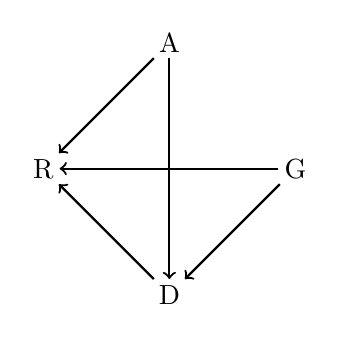
\begin{tikzpicture}[scale=0.8,help lines/.style={color=lightgray,line width=0.2pt},post/.style={->,shorten >=1pt,>=stealth',thick}]
    
    \node[inner sep=2] (A) at (0.0,2.0){A};
    \node[inner sep=2] (G) at (2.0,0.0) {G};
    \node[inner sep=2] (R) at (-2.0,0.0) {R};
    \node[inner sep=2] (D) at (0.0,-2.0) {D};

    \draw[->, thick] (A) -- (R);
    \draw[->, thick] (A) -- (D);
    \draw[->, thick] (G) -- (D);
    \draw[->, thick] (G) -- (R);
    \draw[->, thick] (D) -- (R);
    
    \end{tikzpicture}
    \caption{Belief network}
    \label{fig:all_trade_cca_black}     
\end{figure}

\subsection*{2. Computation of $p(recover \; | \; drug)$}

Applying Bayes rule we get $p(recover \; | \; drug) = \frac{p(recover, \;drug)}{p(drug)}$. This suggests that from a database of patient entries we take the number of patients that both recovered and received the drug and divide it by the number of patients that received the drug. 

\subsection*{2. Computation of $p(recover \; | \; do(drug),\; yound)$}

\section*{Problem 3.11}


\section*{Problem 3.12}


\section*{Problem 3.13}


\section*{Problem 3.14}


\section*{Problem 3.15}


\section*{Problem 3.17}

\subsection*{1.}

In order to prove $a \ci c$ we need to show that $p(a,c) = p(a)p(c)$. We first calculate the joint probability distribution $p(a,b,c) = p(c|b)p(b|a)p(a)$. Then we marginalise over $b$ to get $p(a,c)=\sum_{b} p(a,b,c) = \sum_{b} p(c|b)p(b|a)p(a)$. 

For $b=b_1$ we get $p(b1|a) = \left( \frac{1}{4} \frac{15}{40} \right)$

\section*{Problem 3.20}


\section*{Problem 3.21}


\section*{Problem 3.22}


\section*{Extra Problem A}


\section*{Extra Problem B}


\end{document}
